\begin{figure*}[t]
\centering
\setlength{\tabcolsep}{0.8pt}
\renewcommand{\arraystretch}{0.5}
\newcommand{\cw}{0.131\textwidth}
\begin{tabular}{@{}ccccccc@{}}
\small Test view & \small Ground truth & \small \ours (ours) & \small SSD-GS & \small \gsthree & \small OLAT-GS & \small RNG \\[2pt]
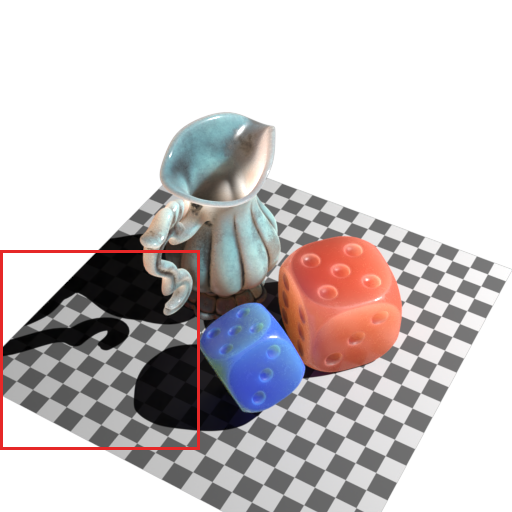
\includegraphics[width=\cw]{figures/comparison/translucent/full.png} & 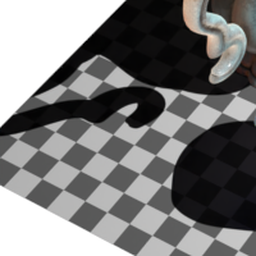
\includegraphics[width=\cw]{figures/comparison/translucent/GT.png} & 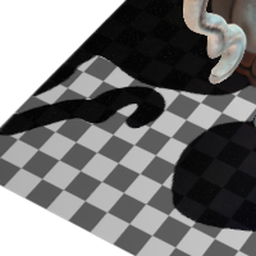
\includegraphics[width=\cw]{figures/comparison/translucent/LiSA-staged.png} & 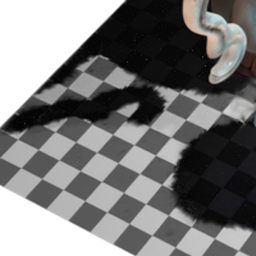
\includegraphics[width=\cw]{figures/comparison/translucent/SSD-GS.png} & 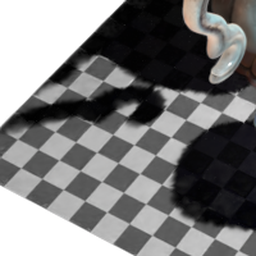
\includegraphics[width=\cw]{figures/comparison/translucent/GS3.png} & 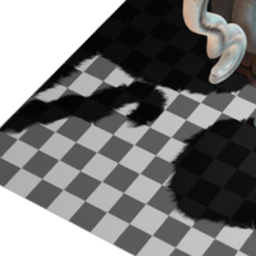
\includegraphics[width=\cw]{figures/comparison/translucent/OLAT-Gaussians.png} & 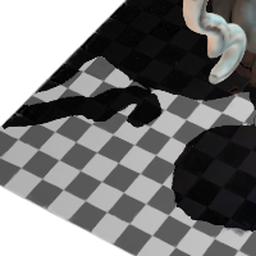
\includegraphics[width=\cw]{figures/comparison/translucent/RNG.png} \\
\footnotesize Translucent & \footnotesize PSNR & \footnotesize \textbf{34.36} & \footnotesize 32.28 & \footnotesize 32.58 & \footnotesize 29.93 & \footnotesize 27.92 \\[3pt]
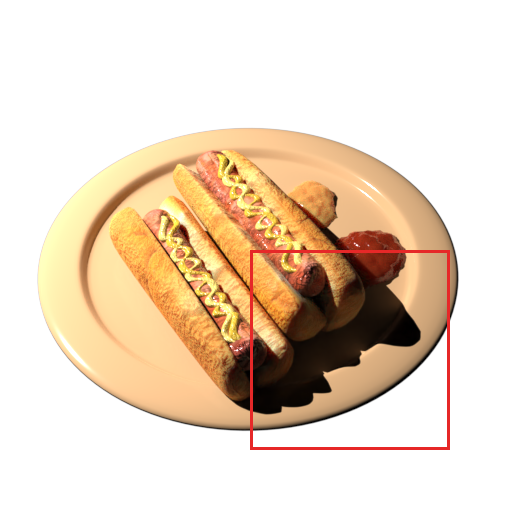
\includegraphics[width=\cw]{figures/comparison/hotdog/full.png} & 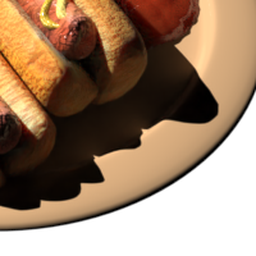
\includegraphics[width=\cw]{figures/comparison/hotdog/GT.png} & 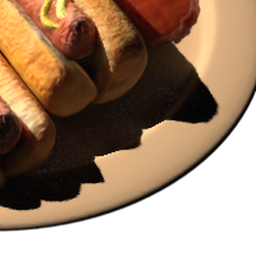
\includegraphics[width=\cw]{figures/comparison/hotdog/LiSA-staged.png} & 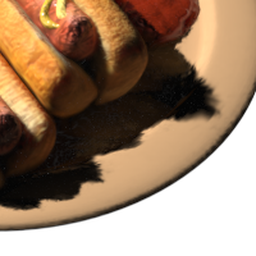
\includegraphics[width=\cw]{figures/comparison/hotdog/SSD-GS.png} & 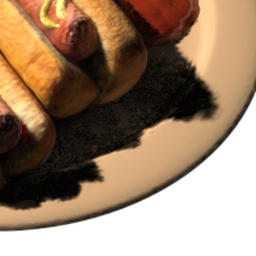
\includegraphics[width=\cw]{figures/comparison/hotdog/GS3.png} & 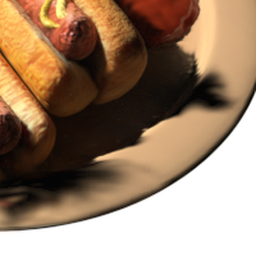
\includegraphics[width=\cw]{figures/comparison/hotdog/OLAT-Gaussians.png} & 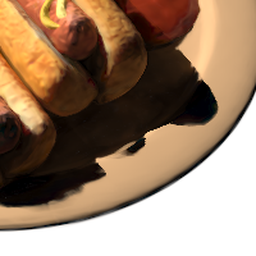
\includegraphics[width=\cw]{figures/comparison/hotdog/RNG.png} \\
\footnotesize Hotdog & \footnotesize PSNR & \footnotesize \textbf{33.97} & \footnotesize 31.93 & \footnotesize 32.08 & \footnotesize 26.85 & \footnotesize 28.49 \\[3pt]
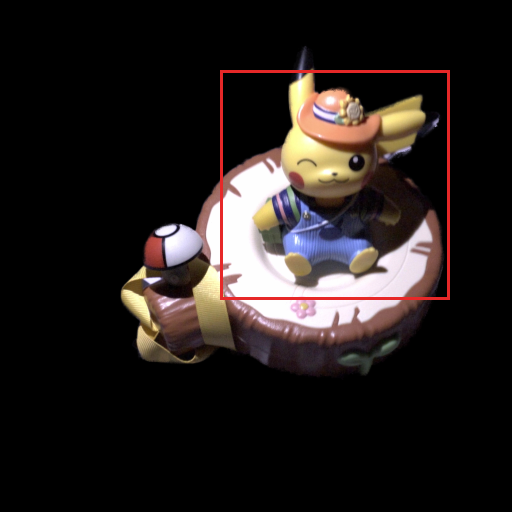
\includegraphics[width=\cw]{figures/comparison/pikachu/full.png} & 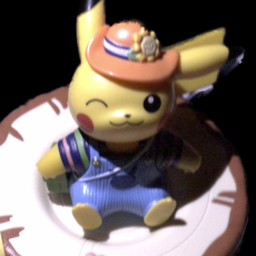
\includegraphics[width=\cw]{figures/comparison/pikachu/GT.png} & 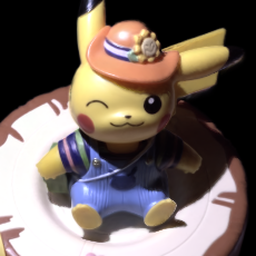
\includegraphics[width=\cw]{figures/comparison/pikachu/LiSA-staged.png} & 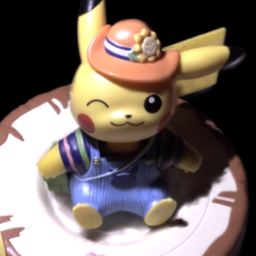
\includegraphics[width=\cw]{figures/comparison/pikachu/SSD-GS.png} & 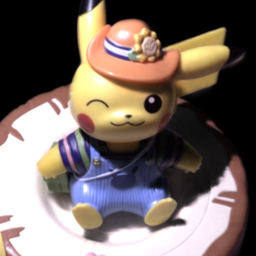
\includegraphics[width=\cw]{figures/comparison/pikachu/GS3.png} & 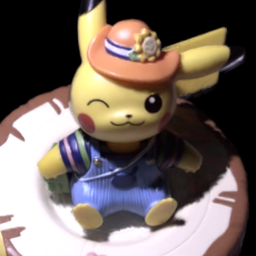
\includegraphics[width=\cw]{figures/comparison/pikachu/OLAT-Gaussians.png} & 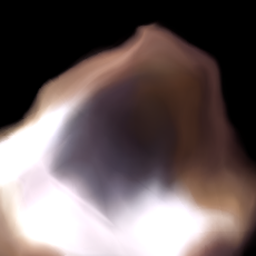
\includegraphics[width=\cw]{figures/comparison/pikachu/RNG.png} \\
\footnotesize Pikachu (real) & \footnotesize PSNR & \footnotesize 30.44 & \footnotesize 29.58 & \footnotesize \textbf{30.71} & \footnotesize 29.46 & \footnotesize 16.31 \\[3pt]
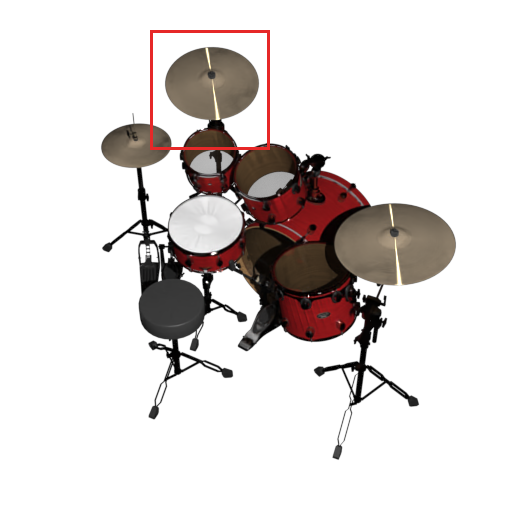
\includegraphics[width=\cw]{figures/comparison/fail_drums/full.png} & 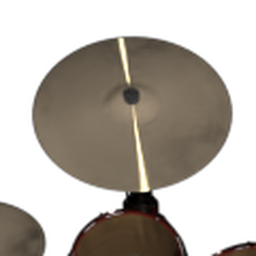
\includegraphics[width=\cw]{figures/comparison/fail_drums/GT.png} & 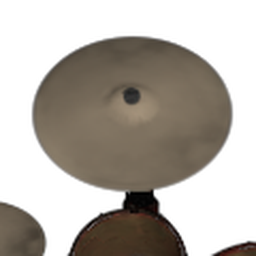
\includegraphics[width=\cw]{figures/comparison/fail_drums/LiSA-staged.png} & 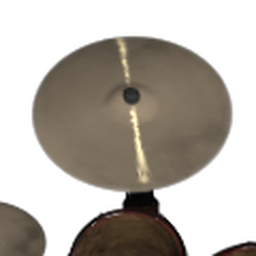
\includegraphics[width=\cw]{figures/comparison/fail_drums/SSD-GS.png} & 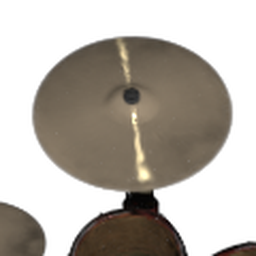
\includegraphics[width=\cw]{figures/comparison/fail_drums/GS3.png} & 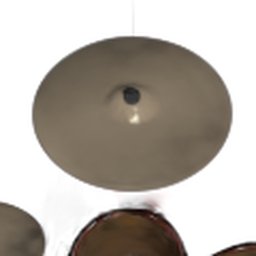
\includegraphics[width=\cw]{figures/comparison/fail_drums/OLAT-Gaussians.png} & 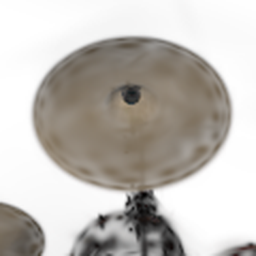
\includegraphics[width=\cw]{figures/comparison/fail_drums/RNG.png} \\
\footnotesize Drums & \footnotesize PSNR & \footnotesize 30.90 & \footnotesize 31.32 & \footnotesize \textbf{31.93} & \footnotesize 22.23 & \footnotesize 16.23 \\[3pt]
\end{tabular}
\caption{\textbf{Qualitative comparison} on test views (crops of the boxed region; PSNR of the full view), each at the median of \ours's per-view margin over the best baseline in its scene. Rows: the two \gsthree scenes dominated by cast shadows, a real capture on which the methods are close, and the synthetic scene where we trail most. Per-primitive shadows of SSD-GS and \gsthree fragment the moving shadows of the vase handle and the hot dogs, which pixel receivers reading the atlas reproduce; \ours misses the thin streak on the Drums cymbal. More scenes, including Fish, are in the supplement.}
\label{fig:comparison}
\end{figure*}
